\begin{frame}
\begin{example}
Where is this function discontinuous?
\begin{columns}[c]
\column{.4\textwidth}
\[
f(x) = \left\{ \begin{array}{lcl}
\frac{x^2 - x - 2}{x-2} & \text{ if } & x \neq 2 \\
\alertNoH{4}{1} & \alertNoH{4}{\text{ if }} & \alertNoH{4}{x = 2} \\
\end{array}\right.
\]
\psset{xunit=0.8cm, yunit=0.8cm}
\begin{pspicture}(-3, -2)(3,4)
\psframe*[linecolor=white](-3,-2)(3,4) \psaxes[labels=none]{<->}(0,0)(-3,-2)(3,4)
\psplot[linecolor=red, plotpoints=1000]{-3}{3}{x 1 add }
\fcHollowDot{2}{3}
\fcFullDot{2}{1}
\end{pspicture} %
%\ 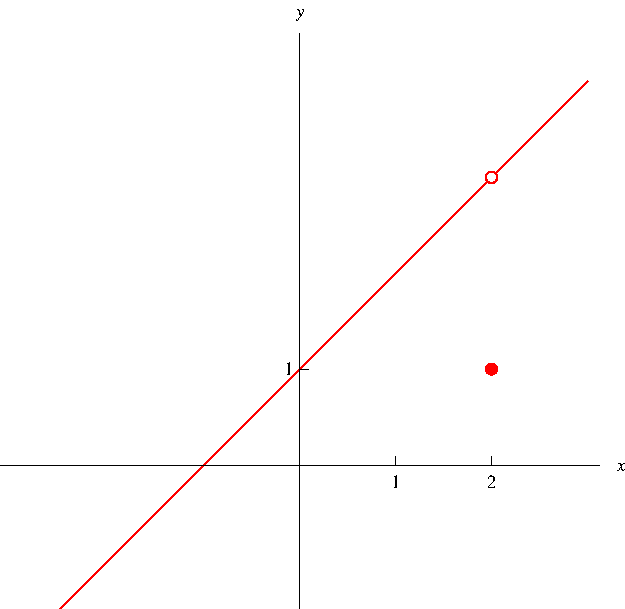
\includegraphics[height=4.5cm]{continuity/pictures/02-05-ex2c.pdf}%
\column{.6\textwidth}
\begin{itemize}
\item<2-| alert@3-4>  $f(2)$ \uncover<4->{is defined ($f(2) = 1$).}
\item<2-| alert@5-6>  $\lim\limits_{x\rightarrow 2} f(x)$ \uncover<6->{exists ($=3$).}
\item<7->  $\lim\limits_{x\rightarrow 2}f(x) \neq f(2)$.
\item<8->  Discontinuous at 2.
\item<9->  This is called a removable discontinuity because we can redefine $f$ at one point to make $f$ continuous.
\end{itemize}
\end{columns}
\end{example}
\end{frame}
